\chapter{Generalizing Newtonian Cosmology}

We begin with a question that is more important than it first sounds: why was it legitimate to use Newton's equations at all in a subject whose proper language is general relativity? Once that point is settled, the lecture moves in two directions. First, we relax the arbitrary assumption of zero total energy and recover the extra \(a^{-2}\) term in Friedmann's equation. Second, we replace slowly moving matter by radiation and discover the different scaling law \(\rho_r \propto a^{-4}\). The result is the standard old cosmological story: a universe that begins radiation dominated, later becomes matter dominated, and only afterward has to be completed by the more modern story of dark energy.

\section{Newton In A Curved Universe}

The lecture opens by backing away from the algebra and asking for a sanity check. Einstein's equations describe curved spacetime, and perhaps curved space as well. Why then should Newton's equations tell us anything reliable about cosmology?

The answer is local. A sufficiently small patch of a curved space looks flat. If we confine attention to neighboring galaxies, or more generally to a region small compared with the radius of curvature of the universe, then Newtonian reasoning is legitimate. The approximation fails only when nearby objects move relativistically with respect to one another, or when we insist on describing the universe on scales large enough that geometry can no longer be ignored.

This is the bridge back to the previous lecture. We have not been studying the whole universe in its full relativistic glory. We have been studying a small comoving patch of it, with nearby matter moving slowly enough that Newton still works. But photons are already warning us that the approximation is incomplete: a homogeneous bath of radiation does move at the speed of light, and that is why the lecture now turns to generalizations.

\section{The Moving Grid And The Matter-Only Universe}

Let us first recall the bookkeeping. We lay down a moving grid on the homogeneous distribution of galaxies and write the physical distance between neighboring grid points as \(a(t)\). The important point is that \(a(t)\) itself is not absolute. If we had chosen a denser or coarser grid, every value of \(a\) would be rescaled by the same constant factor. What survives that ambiguity is the ratio \(\dot a/a\).

If the grid is rescaled by a fixed factor \(\alpha\), then
\begin{align}
a' &= \alpha a, &
\dot a' &= \alpha \dot a,
\end{align}
and therefore
\begin{equation}
\frac{\dot a'}{a'}=\frac{\dot a}{a}.
\end{equation}
That is why the Hubble parameter,
\begin{equation}
H(t)=\frac{\dot a}{a},
\end{equation}
has direct physical meaning, while \(a\) by itself does not yet.

The other useful bookkeeping device is \(\nu\), the mass contained in one comoving unit cell. For ordinary matter, assumed neither created nor destroyed, \(\nu\) is constant in time. The physical density is then
\begin{equation}
\rho=\frac{\nu}{a^3}.
\end{equation}
This is just the statement that the amount of matter in a comoving box stays fixed while the volume of that box grows like \(a^3\).

For the zero-energy matter-only universe, the Newtonian derivation gave
\begin{equation}
\left(\frac{\dot a}{a}\right)^2=\frac{8\pi G}{3}\rho
=\frac{8\pi G}{3}\frac{\nu}{a^3}.
\end{equation}
Because the overall normalization of the grid is arbitrary, we may choose it so that
\begin{equation}
\frac{8\pi G \nu}{3}=1,
\end{equation}
and then the equation takes the simple form
\begin{equation}
\left(\frac{\dot a}{a}\right)^2=\frac{1}{a^3}.
\end{equation}

Now we solve it in the way Susskind solves it on the board. Taking the square root gives
\begin{equation}
\frac{\dot a}{a}=\pm \frac{1}{a^{3/2}},
\end{equation}
so that
\begin{equation}
\dot a=\pm \frac{1}{\sqrt a}.
\end{equation}
On a monotonic branch we may invert the derivative:
\begin{equation}
\frac{dt}{da}=\pm \sqrt a.
\end{equation}
Integrating,
\begin{equation}
t=\pm \frac{2}{3}a^{3/2}+\text{const},
\end{equation}
and therefore, up to the inessential constants that he suppresses in speech,
\begin{equation}
a(t)\propto t^{2/3}.
\end{equation}

This is the matter-dominated, zero-energy solution. It expands forever, but it decelerates. The curve \(a(t)\) flattens out, yet never truly comes to rest.

\begin{figure}
\centering

\includegraphics[width=0.62\textwidth]{lecture_02_figure_02.png}
\caption{Recap of the matter-only solution and the boxed \(a\sim t^{2/3}\) law.}
\end{figure}

\subsection{Question \& Answer}

Why was it permissible to throw away the negative square root when solving the matter-only equation?

The answer is that the equation itself does not decide between expansion and contraction. It only determines \((\dot a/a)^2\). A rock moving radially in the field of a planet can be going out or coming in; Newton's equation does not tell us which branch we are on unless we supply initial conditions. Exactly the same is true here. The positive branch describes an expanding universe; the negative branch describes a contracting one. In the matter-only calculation we chose the expanding branch because that was the physical situation under discussion, not because the equation eliminated the other possibility.

\section{Non-Zero Energy And The Extra Friedmann Term}

The first real generalization is to drop the arbitrary assumption that every galaxy sits exactly at escape velocity. We return to the Newtonian picture: a test galaxy sits at comoving position \(x\), so its physical distance is
\begin{equation}
D=ax,
\end{equation}
and its physical velocity is
\begin{equation}
\dot D=\dot a\,x.
\end{equation}
Susskind simplifies the discussion by taking \(x=1\), so that
\begin{equation}
D=a, \qquad \dot D=\dot a.
\end{equation}

The enclosed mass inside the corresponding sphere is
\begin{equation}
M=\rho \, \frac{4\pi}{3} a^3.
\end{equation}
The Newtonian energy of the test galaxy is then
\begin{equation}
\frac{1}{2}m\dot a^{\,2}-\frac{GMm}{a}=E.
\end{equation}
Divide by \(m\), multiply by \(2\), and absorb the resulting constant on the right into a symbol \(C\):
\begin{equation}
\dot a^{\,2}-\frac{2GM}{a}=C.
\end{equation}
Now divide by \(a^2\):
\begin{equation}
\left(\frac{\dot a}{a}\right)^2-\frac{2GM}{a^3}=\frac{C}{a^2}.
\end{equation}
Using \(M=\rho \frac{4\pi}{3}a^3\), we obtain
\begin{equation}
\left(\frac{\dot a}{a}\right)^2-\frac{8\pi G}{3}\rho=\frac{C}{a^2}.
\end{equation}
Equivalently,
\begin{equation}
\left(\frac{\dot a}{a}\right)^2=\frac{8\pi G}{3}\rho+\frac{C}{a^2}.
\end{equation}

This is the non-zero-energy Friedmann equation in the Newtonian derivation. The extra term remembers whether the total energy was positive or negative.

\begin{figure}
\centering

\includegraphics[width=0.82\textwidth]{lecture_02_figure_03.png}
\caption{Newtonian enclosed-mass sketch and the Friedmann equation for non-zero energy.}
\end{figure}

\begin{figure}
\centering
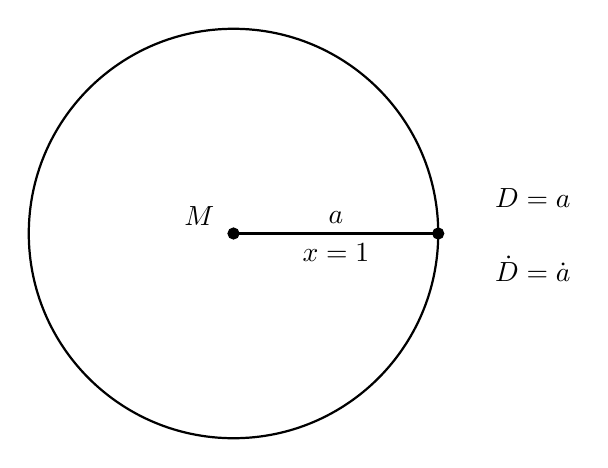
\begin{tikzpicture}[scale=1.0]
\draw[thick] (0,0) circle (2.6);
\filldraw (0,0) circle (2pt);
\node[left] at (-0.12,0.22) {$M$};
\draw[thick] (0,0)--(2.6,0);
\filldraw (2.6,0) circle (2pt);
\node[above] at (1.3,0) {$a$};
\node[below] at (1.3,0) {$x=1$};
\node[right] at (3.2,0.45) {$D=a$};
\node[right] at (3.2,-0.45) {$\dot D=\dot a$};
\end{tikzpicture}
\caption{A clean reconstruction of the enclosed-mass picture used in the \(x=1\) derivation.}
\end{figure}

The lecture does not insist on the full exact solution. Instead it reads the equation by looking at limits.

For very small \(a\), the matter term \(a^{-3}\) dominates the new term \(a^{-2}\). Thus the early universe behaves just as before:
\begin{equation}
a(t)\propto t^{2/3}
\qquad
(a \ \text{small}).
\end{equation}

For \(C>0\), however, the late-time behavior changes. When \(a\) becomes large, the \(a^{-2}\) term beats the \(a^{-3}\) term, and we find
\begin{equation}
\left(\frac{\dot a}{a}\right)^2 \sim \frac{C}{a^2}.
\end{equation}
Taking the positive branch,
\begin{equation}
\dot a \sim \sqrt{C},
\end{equation}
so at late times
\begin{equation}
a(t)\propto t.
\end{equation}
The galaxy has escaped with a margin; once gravity becomes negligible, it coasts outward with approximately constant velocity.

For \(C<0\) the story is different. Write \(C=-|C|\). Then
\begin{equation}
\left(\frac{\dot a}{a}\right)^2
=
\frac{8\pi G}{3}\frac{\nu}{a^3}
-
\frac{|C|}{a^2}.
\end{equation}
At small \(a\), the \(a^{-3}\) term dominates and the universe still expands like \(t^{2/3}\). But at sufficiently large \(a\), the negative \(a^{-2}\) term catches up. The right-hand side can reach zero. That is the turning point: expansion stops, and the universe begins to contract.

\subsection{Question \& Answer}

How can a recollapsing universe arise when \(\left(\dot a/a\right)^2\) is manifestly nonnegative?

This is exactly the point the lecture pauses over. The right-hand side can never become negative; that would indeed be impossible. But it can become zero. If we start on the expanding branch, \(\dot a>0\), then the moment the right-hand side hits zero we have \(\dot a=0\): the universe comes momentarily to rest. After that, the contracting solution takes over, which means choosing the negative square-root branch. So the logic is not that \(\left(\dot a/a\right)^2\) becomes negative. The logic is that it reaches zero at a finite maximum size, and the solution then continues on the negative branch back down.

\section{Geometry On The Left, Energy On The Right}

At this point the lecture changes register. The same Friedmann equation is now read as a stripped-down Einstein equation. Move the \(a^{-2}\) term to the left:
\begin{equation}
\left(\frac{\dot a}{a}\right)^2+\frac{C}{a^2}
=
\frac{8\pi G}{3}\rho.
\end{equation}
This is the form Susskind points to when he says: geometry on the left, source on the right.

\begin{figure}
\centering

\includegraphics[width=0.72\textwidth]{lecture_02_figure_04.png}
\caption{Friedmann equation arranged to match Einstein's geometric and source sides.}
\end{figure}

The lecture also uses a curvature-style notation. If we define
\begin{equation}
K=-C,
\end{equation}
then the same equation becomes
\begin{equation}
\left(\frac{\dot a}{a}\right)^2-\frac{K}{a^2}
=
\frac{8\pi G}{3}\rho.
\end{equation}
This is the form that begins to look familiar from general relativity: the \(a^{-2}\) term is now read as curvature.

\begin{remark}
The board and the spoken lecture slide among \(C\), \(K\), and later \(\kappa\). The clean way to read the discussion is that the Newtonian derivation first produces a raw energy constant \(C\), and then the geometry discussion rewrites the same term with the opposite sign convention in a curvature symbol such as \(K\) or \(\kappa\).
\end{remark}

This is also where the Newtonian mass density is upgraded. On the right-hand side of Einstein's equation it is not merely rest-mass density that matters, but total energy density. With units chosen so that the speed of light is \(1\), we simply write \(\rho\) for the full energy density. Rest mass contributes to it, but so do radiation and any other form of energy present in the universe.

\begin{figure}
\centering

\includegraphics[width=0.84\textwidth]{lecture_02_figure_05.png}
\caption{Curvature form and density-substituted form of the Friedmann equation.}
\end{figure}

The lecture does not yet develop the geometry of space in detail. It only plants the flag: the \(a^{-2}\) term has geometric meaning, and next time that meaning will be unpacked in terms of flat, positively curved, and negatively curved space.

\section{Radiation In An Expanding Box}

Now comes the second generalization. Suppose the universe is filled not with slowly moving massive particles, but with radiation.

The right-hand side of Friedmann's equation must then contain radiation energy density. To understand how that scales, Susskind asks us to look at a single comoving box, one unit cube in the moving grid. Its physical volume is \(a^3\). For ordinary nonrelativistic matter, the energy per particle does not change: the particles simply thin out as the box expands, so the density scales like \(a^{-3}\). Photons are different because their energy depends on wavelength:
\begin{equation}
E_\gamma \propto \frac{1}{\lambda}.
\end{equation}
The key claim is that if the box expands slowly, the wavelength stretches with it:
\begin{equation}
\lambda \propto a.
\end{equation}
Therefore the energy of each photon scales as
\begin{equation}
E_\gamma \propto \frac{1}{a}.
\end{equation}
If the number of photons in the comoving box stays fixed, then the total photon energy in that box goes like \(a^{-1}\). Dividing by the box volume \(a^3\), we find
\begin{equation}
\rho_r \propto \frac{1}{a^4}.
\end{equation}

Insert this into Friedmann's equation:
\begin{equation}
\left(\frac{\dot a}{a}\right)^2
=
\frac{8\pi G}{3}\frac{\nu_r}{a^4}.
\end{equation}
As before, the overall constant can be absorbed by a choice of grid normalization, leaving
\begin{equation}
\left(\frac{\dot a}{a}\right)^2=\frac{1}{a^4}.
\end{equation}
Now solve:
\begin{align}
\frac{\dot a}{a} &= \pm \frac{1}{a^2},\\
\dot a &= \pm \frac{1}{a},\\
\frac{dt}{da} &= \pm a,\\
t &= \pm \frac{1}{2}a^2+\text{const}.
\end{align}
Thus the expanding branch gives
\begin{equation}
a(t)\propto t^{1/2}.
\end{equation}

So the radiation-dominated universe expands more slowly than the matter-dominated one. The two curves look qualitatively similar, but they are not the same, and the difference matters in the thermal history of the early universe.

\subsection{Question \& Answer}

Why should the wavelength of a photon be dragged along by the expanding box at all?

The lecture does not pretend to give a full proof. Instead it gives a piece of wave mechanics intuition. For a standing wave on a slowly changing domain, the number of nodes is an adiabatic invariant. If the size of the domain changes continuously, the node number cannot suddenly jump from one integer to another. The only way to preserve the node count is for the wavelength to readjust to the size of the domain. Susskind imagines a wave on a ring whose circumference is slowly varied: the number of zeros stays fixed, and the wavelength stretches with the ring. The cosmological box is then treated in the same spirit. This is heuristic, but it captures the lesson he wants: slow expansion stretches the wavelength, and stretched wavelength means lower photon energy.

\section{Matter And Radiation Together}

The real universe contains both components. The lecture therefore writes the mixed Friedmann equation as a sum of two source terms,
\begin{equation}
\left(\frac{\dot a}{a}\right)^2
=
\frac{C_m}{a^3}
+
\frac{C_r}{a^4}.
\end{equation}
On the board Susskind first writes the coefficients as \(C_1\) and \(C\), then corrects himself: the radiation term should really carry its own second constant. That is why it is cleaner here to denote the two coefficients by \(C_m\) and \(C_r\).

\begin{figure}
\centering

\includegraphics[width=0.70\textwidth]{lecture_02_figure_06.png}
\caption{Mixed matter-plus-radiation expansion law with \(a^{-3}\) and \(a^{-4}\) terms.}
\end{figure}

The asymptotics are immediate. For small \(a\),
\begin{equation}
\frac{C_r}{a^4} \gg \frac{C_m}{a^3},
\end{equation}
so the radiation term dominates and
\begin{equation}
a(t)\propto t^{1/2}.
\end{equation}
For large \(a\),
\begin{equation}
\frac{C_m}{a^3} \gg \frac{C_r}{a^4},
\end{equation}
so matter dominates and
\begin{equation}
a(t)\propto t^{2/3}.
\end{equation}

This is the old two-component cosmology: the early universe is radiation dominated, then there is a crossover, and afterward the universe behaves like a matter-dominated universe. Dark matter belongs in the matter term. Photons certainly belong in the radiation term, and Susskind also places gravitons and sufficiently light neutrinos there because they move essentially at the speed of light.

\subsection{Question \& Answer}

Are we assuming that matter and radiation are separately conserved?

Yes, approximately, and the lecture says so explicitly. The assumption is that once the universe cools enough, matter and radiation no longer exchange energy efficiently. The photons free-stream, scatter less and less, and each component is then well described by its own nearly time-independent coefficient. This is not the last word, but it is good enough for the cosmological epoch under discussion.

The lecture also pauses over observation. We do not directly see galaxies in the era when \(a(t)\propto t^{1/2}\), because that comes before galaxies formed. But the early thermal history still remembers it. Nucleosynthesis, the microwave background, and the general temperature history of the universe are sensitive to the radiation-dominated phase. The matter-dominated law \(t^{2/3}\) is easier to see directly; the radiation-dominated law is inferred more indirectly, but the lecture insists that the evidence for it is nonetheless substantial.

\section{Loose Ends And Forward Pointers}

The lecture closes by refusing to over-promise. Several natural questions are raised and only partly answered.

One concerns the fate of the energy lost by photons as the universe expands. The quick answer is that the radiation does work on the expanding box. That is easy to say in a literal box with walls; in cosmology the statement becomes more subtle, because the ``box'' is really the expanding grid itself. Susskind is content, for the moment, to say that this can still be analyzed as an expanding-box problem, and that a more careful discussion of energy conservation in general relativity must wait.

A second concerns superluminal recession. If
\begin{equation}
v=HD,
\end{equation}
then sufficiently large \(D\) implies \(v>1\) in units where the speed of light is \(1\). The lecture's answer is that this does not contradict relativity in the naive way one might think. It is not the same as watching a nearby object pass by faster than light, and it is tied instead to the geometry of the expanding universe and to the notion of horizons.

A third concerns curvature. The \(a^{-2}\) term is said to know about spatial geometry, but the geometries themselves are deferred to the next lecture: flat space, positively curved space, and negatively curved space.

Finally, the lecture reminds us that even this two-component universe is not the final story. It is, as Susskind says, the cosmology of thirty years ago. The next layer is dark energy.

\section{Summary}

The lecture takes the Newtonian cosmology of the previous discussion and makes it more serious in two ways. First, it drops the arbitrary zero-energy assumption and recovers the extra \(a^{-2}\) term, whose sign determines whether the universe expands forever or eventually recollapses. Second, it replaces rest-mass density by total energy density and shows that radiation scales differently from matter because photon energies redshift as wavelengths stretch.

The resulting picture is simple and powerful. Matter gives \(\rho_m\propto a^{-3}\) and \(a\propto t^{2/3}\). Radiation gives \(\rho_r\propto a^{-4}\) and \(a\propto t^{1/2}\). In a universe containing both, radiation dominates first and matter later. Beyond that point lie the questions the lecture deliberately postpones: curvature, horizons, and dark energy, where the full geometry of general relativity finally has to take over.